\section{Openflow}



\subsection{Definição}

Em 2008 o protocolo OpenFlow foi publicado. Ele permitiu que pesquisadores
pudessem criar experimentos com novos protocolos em redes convencionais
\citep{nick2008openflow}.
O OpenFlow foi criado como um padrão aberto, o que permite que todos os 
fabricantes de equipamentos de redes possam habilitar seus produtos a esse 
padrão.

O protocolo consiste em uma interface de programação para o switch. 
Assim, um programador pode, através de um programa, controlar a forma como 
um switch executa seu encaminhamento de pacotes. 
De uma maneira bem clara, o protocolo OpenFlow separa o plano de dados
do plano de controle, fazendo com que soluções SDN possam ser criadas 
e experimentadas.
Por ser uma solução de baixo custo, o OpenFlow obteve boa aceitação na 
academia e no mercado, dado o volume de empresas e pesquisas relacionadas
ou que utilizam o protocolo.

\subsection{Componentes}

Na arquitetura estabelicida pelo protocolo OpenFlow existem dois papéis
principais.
O controlador e o switch OpenFlow. 
Uma separação baseada no modelo das Redes definidas por software (SDN)
conforme pode ser visto na figura~\ref{fig:of-arch}.

\begin{figure}[h!]
    \centering
    \label{fig:of-arch}
    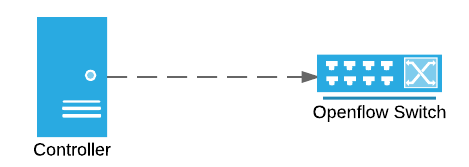
\includegraphics{img/openflow-architecture}
    \caption{Divisão da arquitetura OpenFlow}
\end{figure}

\subsection{Arquitetura do Switch}

O switch OpenFlow pode ser dividido em três principais partes. 
A primeira é o canal de comunicação seguro com o controlador.
A segunda é a interface do protocolo OpenFlow que permite ao controlador
controlar o switch.
A terceira é sua tabela de fluxos.

O canal de comunicação seguro tem a garantia de confiabilidade na troca 
de mensagens entre o controlador e o switch através do protocolo SSL 
(Secure Socket Layer). 
Isso adiciona proteção à rede em relação a ataques de elementos mal 
intencionados \citep{rothenberg2010openflow}.

A interface do protocolo OpenFlow é a padronização das mensagens enviadas 
pelo controlador ao switch de modo a definir o comportamento do encaminhamento
de pacotes. 
Ou seja, é o conjunto de possíveis instruções para se controlar de maneira
genérica o plano de dados de qualquer \emph{hardware} de redes habilitado 
ao padrão OpenFlow.

A tabela de fluxos é composta por regras.
Cada regra consiste em ações associadas à fluxos. 
Através dessa tabela o switch executa o encaminhamento de pacotes. 
As entradas dessa tabela são atualizadas pelo controlador.

\begin{figure}[h!]
    \centering
    \label{fig:switch-arch}
    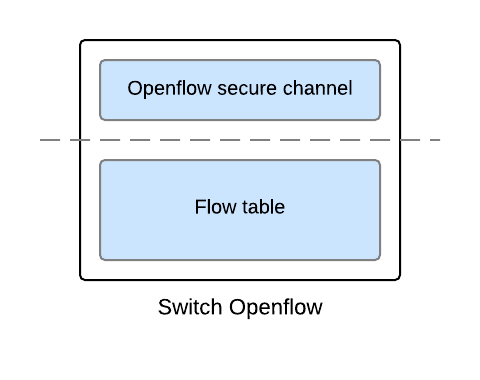
\includegraphics[width=\linewidth]{img/switch-architecture}
    \caption{Arquitetura do switch OpenFlow}
\end{figure}


\subsection{Fluxos}

Um fluxo é a representação de um ou mais pacotes em função de suas
características.
Essas características variam de acordo com o cabeçalho OpenFlow.
Os fluxos são genéricos. 
Ao invés de avaliar pacotes e portas para fazer a análise do trafego,
que representam o passado, os fluxos representam futuro. 
Um fluxo pode caracterizar pacotes que ainda não passaram pelo switch mas 
que possuem as mesmas características que compõem aquele fluxo. 
Sendo assim, a ação associada ao fluxo é aplicada a esses novos pacotes.


\begin{table}[h!]
    \centering
    \begin{tabular}{| l | l |}
    \hline
    \textbf{Contador} & \textbf{Bits} \\ \hline
    Pacotes Recebidos & 64 \\ \hline
    Pacotes Transmitidos & 64 \\ \hline
    Bytes Recebidos & 64 \\ \hline
    Bytes Transmitidos & 64 \\ \hline
    Drops Recebidos & 64 \\ \hline
    Drops Transmitidos & 64 \\ \hline
    Erros Recebidos & 64 \\ \hline
    Erros Transmitidos & 64 \\ \hline
    Erros de Frames Recebidos & 64 \\ \hline
    Erros de Transbordo Transmitidos & 64 \\ \hline
    Erros de CRC Recebidos & 64 \\ \hline
    Colisões & 64 \\
    \hline
    \end{tabular}
    \caption{Contadores de fluxos por Porta}
    \label{tbl:counters}
\end{table}



A tabela de fluxos dentro do switch OpenFlow identifica os fluxos para que o 
plano de dados execute ações sobre os pacotes que são pertencentes àquele
fluxo. 
A tabela \ref{tbl:flowtable} apresenta de maneira simplificada a tabela 
de fluxos dentro do switch OpenFlow.

\subsection{Cabeçalho}

O cabeçalho OpenFlow se estende da camada 1 até a camada 4 da pilha TCP/IP.
A figura \ref{fig:of-header} apresenta os campos e suas respectivas camadas.

\begin{figure}[h!]
    \centering
    \label{fig:of-header}
    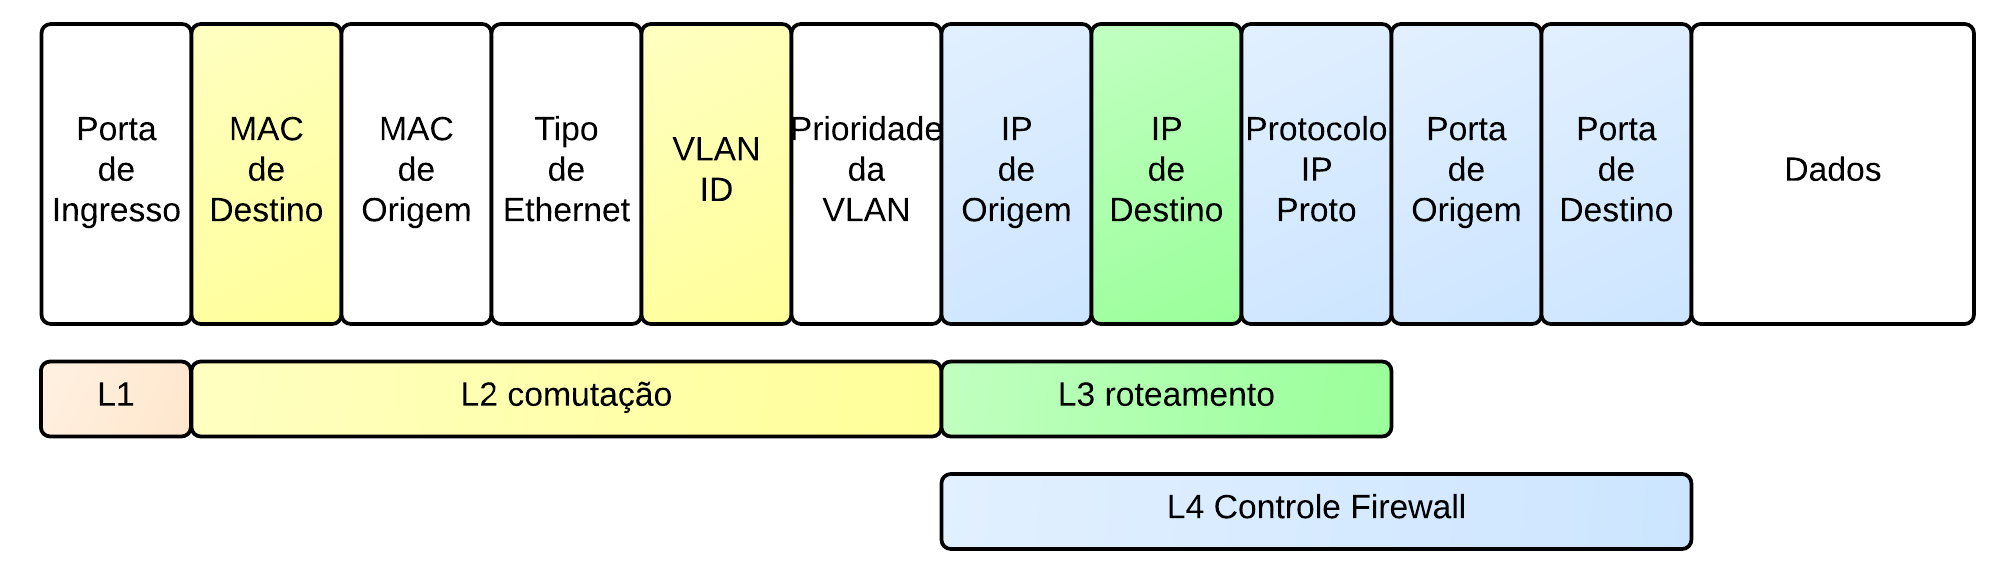
\includegraphics[width=\linewidth]{img/openflow-header}
    \caption{Cabeçalho OpenFlow}
\end{figure}

Quando um novo pacote ingressa no switch OpenFlow esse cabeçalho é preenchido
e encaminhado para o controlador. 
Através da análise dessas informações do fluxo o controlador envia uma 
mensagem ao switch instalando/atualizando regras na tabela de fluxos. 

Esse mecanismo de rotulagem e identificação de tráfego e pacotes (fluxos) é
inspirado no MPLS (\emph{Multi-protocol Label Switching}) 
\citep{bruce2008mpls}.

\subsection{Ações}

As ações (\emph{actions}) são aplicadas aos fluxos especificados na tabela
de fluxos do switch.
Ações como encaminhamento, atualização de cabeçalho e rejeição podem ser 
aplicadas aos pacotes pertencentes àquele fluxo.

A especificação do protocolo OpenFlow \citep{ofprotocol2015} descreve todas 
as possíveis ações que podem ser aplicadas.
A lista abaixo apresenta algumas ações:

\begin{multicols}{3}
    \begin{itemize}
        \item Forwarding
        \item Drop
        \item Set
        \item Strip
        \item Copy-in
        \item Copy-out
        \item Push
        \item Pop
        \item Dec
    \end{itemize}
\end{multicols}

Essas ações são aplicadas a cada novo pacote pertencente ao algum determinado
fluxo pertencente à tabela de fluxos.

\subsection{Controlador}

O controlador é a entidade na rede que representa o plano de controle dentro
da arquitetura OpenFlow.
Apesar de ser um entidade logicamente centralizada, ele pode ser distribuído.
O controlador é um software que se conecta de maneira segura ao switch 
OpenFlow.
Através da interface de programação do protocolo o controlador manipula 
a tabela de fluxos do switch.

Em função dessa arquitetura, é possível ter visão e controle de estado global
da rede.
Como o protocolo OpenFlow especifica que o switch armazena alguns dados 
estatísticos, por exemplo de portas e fluxos, o controlador pode tomar 
decisões ou executar análises sobre a rede baseando-se nessas estatísticas.

O controlador exerce um papel importante para os serviços em execução dentro
da rede. 
Outros servidores rodando aplicações podem fazer requisições e troca de 
mensagens com o controlador da rede, de modo a obter informações topológicas
ou de estado da rede.

Com o plano de controle isolado em uma aplicação logicamente centralizada, 
um programador tem de lidar com problemas típicos de desenvolvimento de 
software e sistemas distribuídos como:

\begin{itemize}
    \item Tolerância a falhas
    \item Persistência
    \item Eficiência
    \item Design de implementação
    \item Debugging
    \item Testes
\end{itemize}

Existem vários softwares controladores \emph{open source} no mercado que 
podem ser utilizados em produção em para desenvolvimento de pesquisas:

\begin{itemize}
    \item Biblioteca \href{http://opennetworkingfoundation.github.io/libfluid/index.html}{Libfluid}
        para criação de aplicações/controladores em SDN \citep{libfluid2015}
    \item \href{http://www.noxrepo.org/nox/about-nox/}{Nox Controller}
        \citep{nox2015}
    \item \href{https://openflow.stanford.edu/display/Beacon/Home}{Beacon}
        \citep{beacon2015}
    \item \href{http://www.noxrepo.org/pox/about-pox/}{Pox Controller}
        \citep{pox2015}
    \item \href{http://osrg.github.io/ryu/}{Ryu} \citep{ryu2015}
\end{itemize}

